\documentclass[11pt,a4paper]{article}

\usepackage[top=2.0cm, bottom=2.0cm, left=2.2cm, right=2.2cm]{geometry}
\usepackage{amsmath, amssymb}
\usepackage{graphicx}
\usepackage{booktabs}
\usepackage{hyperref}
\usepackage{natbib}
\usepackage{microtype}
\usepackage[T1]{fontenc}
\usepackage{lmodern}
\usepackage{parskip}
\setlength{\parskip}{2pt}
\setlength{\abovecaptionskip}{4pt}
\setlength{\belowcaptionskip}{0pt}

\hypersetup{colorlinks=true, linkcolor=blue, citecolor=blue, urlcolor=blue}

\title{\textbf{The Interaction Between Synaptic Noise and Intrinsic\\
Excitability in Representational Drift}\\[0.5em]
\large Computational Neuroscience \textemdash{} Final Project}

\author{Elena Egorova (903570273) \and Sara Bezrukavnikov (905708657)}
\date{April 2026}

\begin{document}
\maketitle
\thispagestyle{empty}

% ================================================================
\begin{abstract}
Hebbian plasticity encodes memories as weight changes in recurrent networks, yet
memories remain vulnerable when network activity is suppressed by anesthesia or
deep inhibition.  We implement a minimal rate-based recurrent network ($N=10$)
with an all-inhibitory structural baseline ($W_\mathrm{struct}\leq 0$), Hebbian
weight plasticity, per-neuron intrinsic excitability ($\varepsilon_i$), and
homeostatic mean-rate regulation, and simulate a three-day equal-duration protocol
(20\,s each) across four conditions: a \emph{Baseline} (no noise),
\emph{Condition~A} (synaptic noise), \emph{Condition~B} (slow intrinsic
excitability fluctuations), and \emph{Condition~C} (both).
All conditions share an identical encoding phase (Day~1, 20\,s).
During suppression (Day~2, 20\,s, $I_p=-3$), the ReLU nonlinearity silences
Hebbian updates; the trace decays passively to $\approx37\%$ of its Day~1 value.
On Day~3 (20\,s), homeostasis overcomes the suppressive input and restores firing.
The key finding is a \emph{stochastic bifurcation} introduced by excitability
fluctuations: Baseline and Condition~A produce a deterministic, reproducible
recovery ($m_\mathrm{mem}\approx1.1$, $\mathrm{std}\approx0$), whereas Conditions
B and C show high outcome variability ($\mathrm{std}\approx0.74$) across random
seeds---the network can converge to either the correct memory attractor or a
spurious one depending on the specific excitability trajectory.
Synaptic noise alone does not alter mean recovery or its variance.
\end{abstract}

% ================================================================
\section{Introduction}

Cortical circuits must encode memories during learning while keeping those
memories stable during retrieval.  Hebbian plasticity---the strengthening of
connections between co-active neurons---provides a mechanism for encoding
\citep{Rule2019}, but the stored trace is vulnerable to any perturbation that
silences activity: anesthesia, deep sleep, or strong inhibitory drive halts
potentiation and allows passive weight decay toward the structural baseline.

Whether a memory trace survives suppression, and whether it can subsequently be
``rescued'' by homeostatic regulation, depends on at least two factors that have
not been studied jointly: (1)~synaptic noise, which adds stochasticity to weight
dynamics and may erode the trace even when activity is suppressed; and (2)~slow
fluctuations in intrinsic excitability \citep{Delamare2023}, which shift
individual neurons' thresholds for reactivation and may bias the pattern of
recovery toward or away from the encoded assembly.

Here we implement a minimal rate-based network and ask: how do synaptic noise
and excitability fluctuations, separately and jointly, affect the integrity of a
Hebbian memory trace and the fidelity of its homeostatic rescue, and how
reproducible are these effects across random noise realizations?

% ================================================================
\section{Methods}

\subsection{Network model}

We simulate $N = 10$ rate units governed by

\begin{equation}
\tau_r\,\dot{r}(t) = -r(t) + W(t)\,\phi(r(t)) + I(t) + \varepsilon + h,
\label{eq:rate}
\end{equation}

where $\phi = \mathrm{ReLU}$, $\varepsilon\in\mathbb{R}^N$ is a per-neuron
excitability bias (zero in Baseline and A), and $h$ is a scalar homeostatic
drive (active only on Day~3).  The structural weight baseline
$W_\mathrm{struct}$ is entirely inhibitory: all entries drawn from
$-\mathrm{Uniform}(0,W_s/N)$, diagonal set to zero.  Recurrent weights evolve by

\begin{equation}
\tau_W\,\dot{W}(t) = -\lambda\bigl(W(t) - W_\mathrm{struct}\bigr)
                    + \eta\,\phi(r)\,\phi(r)^\top,
\label{eq:weights}
\end{equation}

and the homeostatic variable follows

\begin{equation}
\tau_h\,\dot{h}(t) = \kappa\bigl(m^* - m_\mathrm{mean}(t)\bigr),
\qquad m_\mathrm{mean} = \tfrac{1}{N}\mathbf{1}^\top r.
\label{eq:homeo}
\end{equation}

All parameters are in Table~\ref{tab:params}.  Equations are integrated with
simultaneous Euler steps of $dt = 10$\,ms: $\dot{r}$ and $\dot{W}$ are computed
from the \emph{same} $r(t)$, $W(t)$ before any update.

\begin{table}[h]
\centering
\small
\begin{tabular}{llr}
\toprule
Symbol & Meaning & Value \\
\midrule
$N$         & Number of neurons         & 10 \\
$\tau_r$    & Rate time constant        & 10 ms \\
$\tau_W$    & Weight time constant      & 2000 ms \\
$\tau_h$    & Homeostasis time constant & 500 ms \\
$\eta$      & Hebbian learning rate     & 0.005 \\
$\lambda$   & Weight decay rate         & 0.1 \\
$\kappa$    & Homeostatic gain          & 0.2 \\
$m^*$       & Target mean rate          & 0.5 \\
$W_s$       & Structural weight scale   & 0.1 \\
$dt$        & Euler step size           & 10 ms \\
\bottomrule
\end{tabular}
\caption{Model parameters.}
\label{tab:params}
\end{table}

\subsection{Three-day protocol}

All three days have equal duration of 20\,s (2000 Euler steps each).

\paragraph{Day 1 \textemdash{} encoding (20\,s).}
A sparse cue $I_\mathrm{base}\in\mathbb{R}^N$ activates five neurons
(indices $\{0,3,4,5,7\}$, amplitudes $0.85$--$1.48$) for 20\,s.
No homeostasis; $\varepsilon = 0$.  Hebbian plasticity accumulates a memory
trace $\Delta W = W - W_\mathrm{struct}$.  The encoding is identical across
all four conditions.

\paragraph{Day 2 \textemdash{} suppression (20\,s).}
A uniform negative input $I_p = -3\,\mathbf{1}$ drives all rates below zero,
silencing the Hebbian term via ReLU.  Weights decay passively toward
$W_\mathrm{struct}$ by the factor $\exp(-\lambda t/\tau_W) = e^{-1} \approx 0.37$.
Homeostasis is off.

\paragraph{Day 3 \textemdash{} homeostatic rescue (20\,s).}
$I_p$ \emph{remains active} while homeostasis turns on.  The drive $h(t)$
rises to overcome the suppressive input and restore mean firing rates.
Conditions differ by the presence/absence of synaptic noise and
excitability fluctuations during Days~2 and~3.

\subsection{Four conditions}

All conditions start Day~2 from the identical Day~1 final state
($W_\mathrm{d1}$, $r_\mathrm{d1}$).

\begin{itemize}\setlength\itemsep{1pt}
\item \textbf{Baseline}: no noise ($\sigma_\eta=0$), $\varepsilon=0$.
\item \textbf{A -- synaptic noise}: each weight update includes an i.i.d.\
  Gaussian term, so Eq.~\eqref{eq:weights} becomes
  $\tau_W\,\dot{W} = -\lambda(W-W_\mathrm{struct}) + \eta\,\phi(r)\phi(r)^\top
  + \sigma_\eta\,\xi(t)$,
  with $\sigma_\eta = 0.01$ and $\xi_{ij}(t)\sim\mathcal{N}(0,1)$ i.i.d.;
  $\varepsilon=0$.
\item \textbf{B -- excitability}: each $\varepsilon_i$ follows an
  Ornstein--Uhlenbeck process
  \begin{equation}
    \tau_\varepsilon\,d\varepsilon_i = -\varepsilon_i\,dt
      + \sigma_\varepsilon\sqrt{2\,dt/\tau_\varepsilon}\;\xi_i(t),
    \label{eq:ou}
  \end{equation}
  with $\tau_\varepsilon=1000$\,ms, $\sigma_\varepsilon=0.8$,
  $\xi_i\sim\mathcal{N}(0,1)$; no synaptic noise.
\item \textbf{C -- both}: synaptic noise \emph{and} excitability fluctuations
  as above.
\end{itemize}

\subsection{Analysis}

The primary readout is the memory projection
$m_\mathrm{mem}(t) = r_m \cdot r(t)/\|r_m\|$
where $r_m$ is the Day~1 final pattern.  We also track the homeostatic drive
$h(t)$, the mean firing rate $m_\mathrm{mean}(t)$, and the Hebbian trace norm
$\|\Delta W\|_1/N^2$.

To assess reproducibility, we run each condition with $n=20$ independent random
seeds (controlling the noise and OU trajectories in Days~2--3 only; Day~1
encoding is always deterministic).  We report mean $\pm$ std of $m_\mathrm{mem}$
at the end of Day~3.

% ================================================================
\section{Results}

\subsection{Day 1: Hebbian weight buildup from an all-inhibitory baseline}

During the 20\,s encoding period, the five active neurons sustain firing rates
near $\bar{r}\approx 0.77$; the remaining five are silent (Figure~\ref{fig:day1}a).
Because $\tau_r \ll \tau_W$, rates reach quasi-steady state almost instantly and
Hebbian plasticity slowly accumulates the outer product $\phi(r)\phi(r)^\top$.

Figure~\ref{fig:day1}b--d shows $\Delta W = W - W_\mathrm{struct}$ at $t\approx7$,
13, and 20\,s.  The weight change is approximately rank-1: a block of excitatory
entries grows among the five co-active neurons while all other pairs remain in the
inhibitory structural baseline (see also Figure~\ref{fig:Wgrid}, Day~1 column).

\begin{figure}[h]
\centering
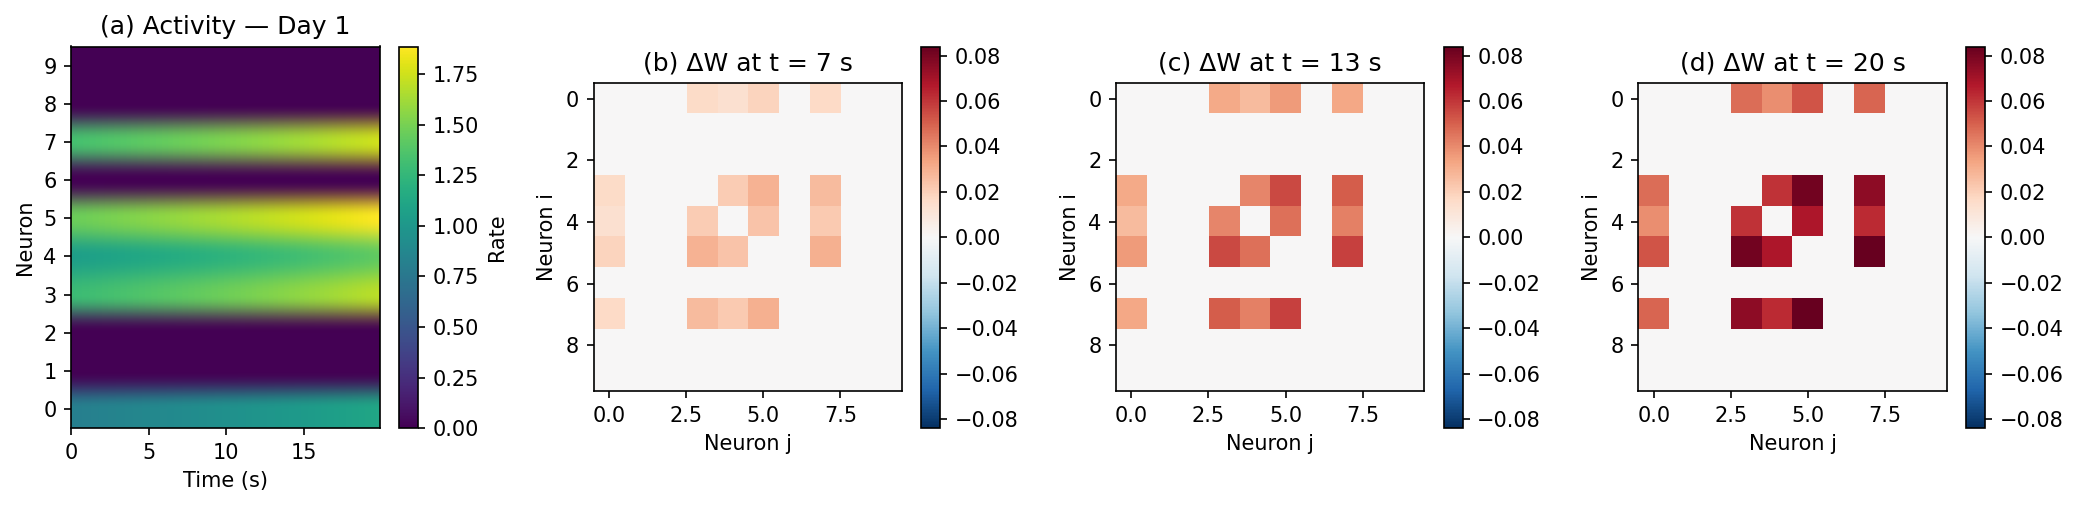
\includegraphics[width=0.97\linewidth, height=4.2cm, keepaspectratio]{../figures/fig_report1.png}
\caption{\textbf{Day 1 memory encoding.}
(a)~Firing-rate heatmap (neuron $\times$ time) during the 20\,s encoding period.
(b--d)~Weight change $\Delta W = W - W_\mathrm{struct}$ at $t\approx7$, $13$, $20$\,s.
Red entries show growing Hebbian potentiation among the five co-active neurons;
the all-inhibitory baseline is preserved elsewhere.}
\label{fig:day1}
\end{figure}

\subsection{Day 2: passive trace decay under suppression}

The negative input $I_p=-3$ immediately drives all rates below zero.
Because $\phi(r)=0$, the Hebbian term vanishes identically in all four conditions.
The trace decays passively to $\approx37\%$ of its Day~1 value in Baseline and B,
consistent with $\exp(-\lambda t/\tau_W) = e^{-1} \approx 0.37$ for $t=20$\,s.
Noise conditions (A, C) retain slightly more trace ($\approx43\%$): because
$\phi(r)=0$ during Day~2, the noise term $\sigma_\eta\xi(t)$ adds zero-mean
stochastic fluctuations that increase the Frobenius norm without systematic
directional bias.

\subsection{Day 3: stochastic bifurcation driven by excitability}

With $I_p$ still active and homeostasis on, $h(t)$ rises toward $\approx3.5$
in all conditions (Figure~\ref{fig:dynamics}b).  After the homeostatic threshold
is crossed, recurrent dynamics and the residual Hebbian trace determine which
neurons reactivate and in what order.

The central finding emerges from repeating each condition across 20 independent
noise realizations (Figure~\ref{fig:robustness}).  \textbf{Baseline} and
\textbf{Condition~A} produce entirely deterministic outcomes:
$m_\mathrm{mem} = 1.10 \pm 0.00$ and $1.10 \pm 0.00$, respectively.
The scalar homeostatic drive lifts all neurons symmetrically, and the Hebbian
trace reliably selects the correct assembly.  Synaptic noise at $\sigma_\eta=0.01$
has no measurable effect on either the mean or the variance.

\textbf{Conditions~B and~C}, by contrast, show high outcome variability:
$m_\mathrm{mem} = 0.96 \pm 0.74$ and $0.96 \pm 0.74$, respectively.
The OU excitability process $\varepsilon_i$ introduces neuron-specific
reactivation thresholds: on Day~3, neuron $i$ crosses zero when
$h(t) > |I_p| - \varepsilon_i(t)$.  If a non-assembly neuron happens to have
large $\varepsilon_i > 0$ at the moment of reactivation, it activates before
assembly neurons and recruits Hebbian potentiation, creating a competing weight
pattern.  Whether the assembly or its competitors reactivate first depends
entirely on the specific OU trajectory---hence the large variance.

A single illustrative trajectory (Figures~\ref{fig:dynamics}--\ref{fig:activity})
shows both extremes: Condition~B can yield $m_\mathrm{mem}=2.89$ (assembly
reactivates first and gets strongly reinforced) while Condition~C yields
$m_\mathrm{mem}=1.24$ (partial competition).

\begin{figure}[h]
\centering
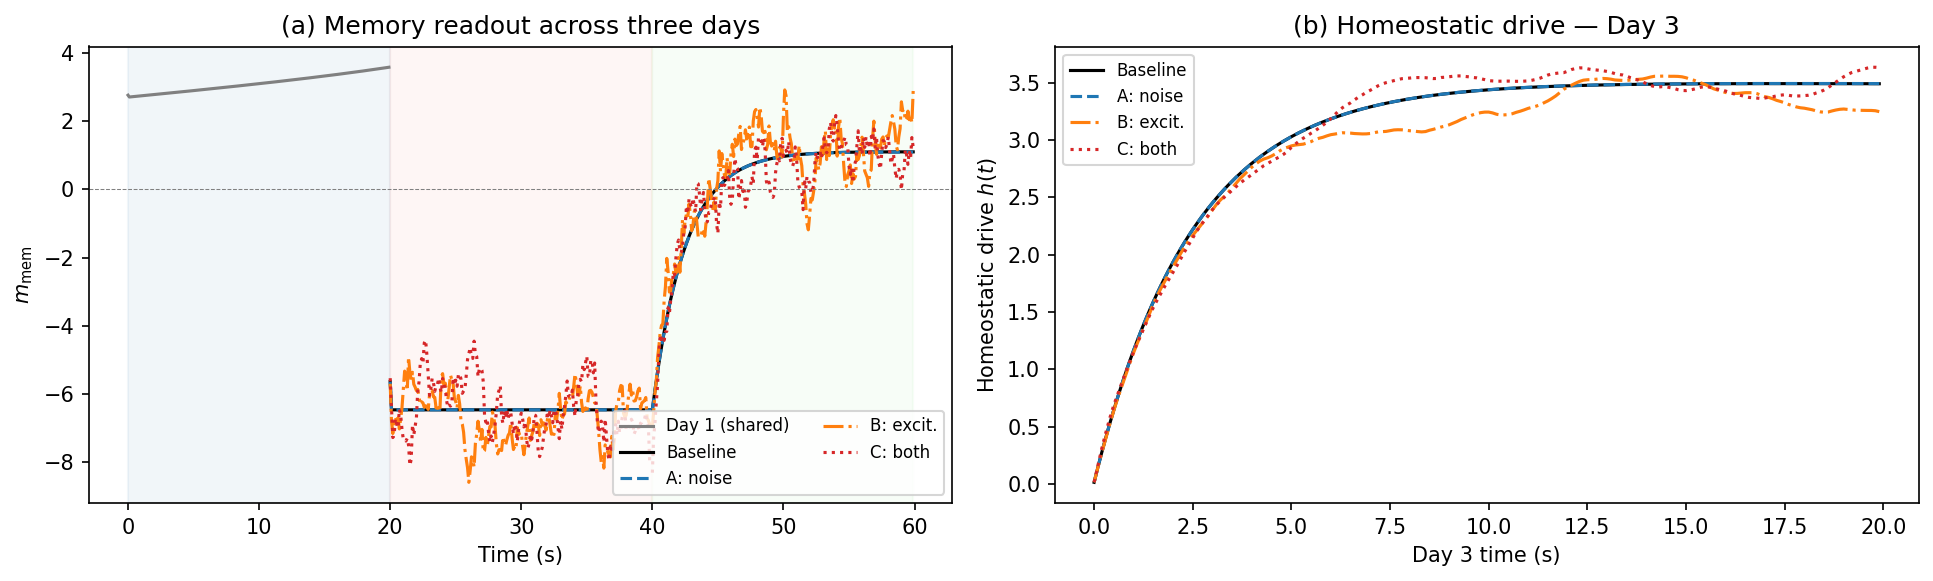
\includegraphics[width=0.97\linewidth, height=4.4cm, keepaspectratio]{../figures/fig_report2.png}
\caption{\textbf{Three-day dynamics across four conditions (one seed).}
(a)~Memory readout $m_\mathrm{mem}(t)$ across the three days for seed 42.
(b)~Homeostatic drive $h(t)$ during Day~3: all conditions reach $h\approx3.5$
to overcome $I_p=-3$.}
\label{fig:dynamics}
\end{figure}

\begin{figure}[h]
\centering
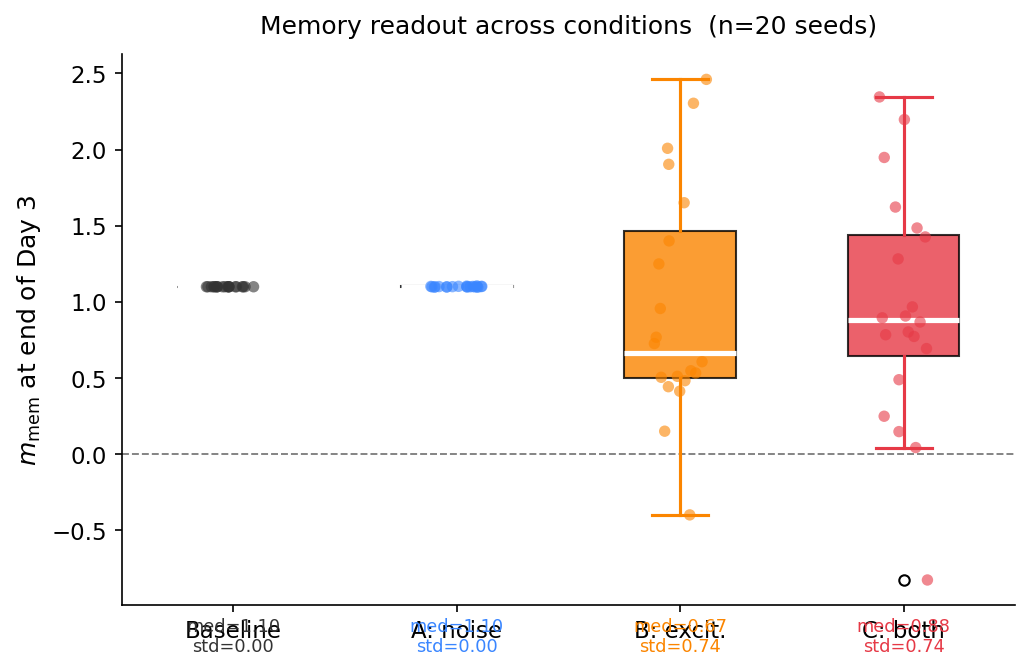
\includegraphics[width=0.85\linewidth]{../figures/fig_robustness.png}
\caption{\textbf{Stochastic bifurcation in memory recovery across 20 independent noise
realizations.}
Box-and-whisker plot of $m_\mathrm{mem}$ at the end of Day~3 for each condition
($n=20$ seeds; individual data points overlaid as circles).
White line: median; box: IQR; whiskers: 1.5$\times$IQR; tick labels show median
and std.
Baseline and Condition~A produce fully deterministic outcomes
($\mathrm{med}=1.10$, $\mathrm{std}=0.00$): the residual Hebbian trace alone
determines recovery regardless of the noise realization.
Conditions~B and~C show a stochastic bifurcation ($\mathrm{std}\approx0.74$):
outcomes span from failed recovery ($m_\mathrm{mem}<0$) to strong reinforcement
($m_\mathrm{mem}>2$), depending on which neurons happen to have the largest
excitability $\varepsilon_i$ at the moment of homeostatic reactivation.
Adding synaptic noise (A vs.\ Baseline; C vs.\ B) shifts neither the median nor
the variance, confirming that the bifurcation is driven exclusively by the OU
excitability process.}
\label{fig:robustness}
\end{figure}

\begin{figure}[h]
\centering
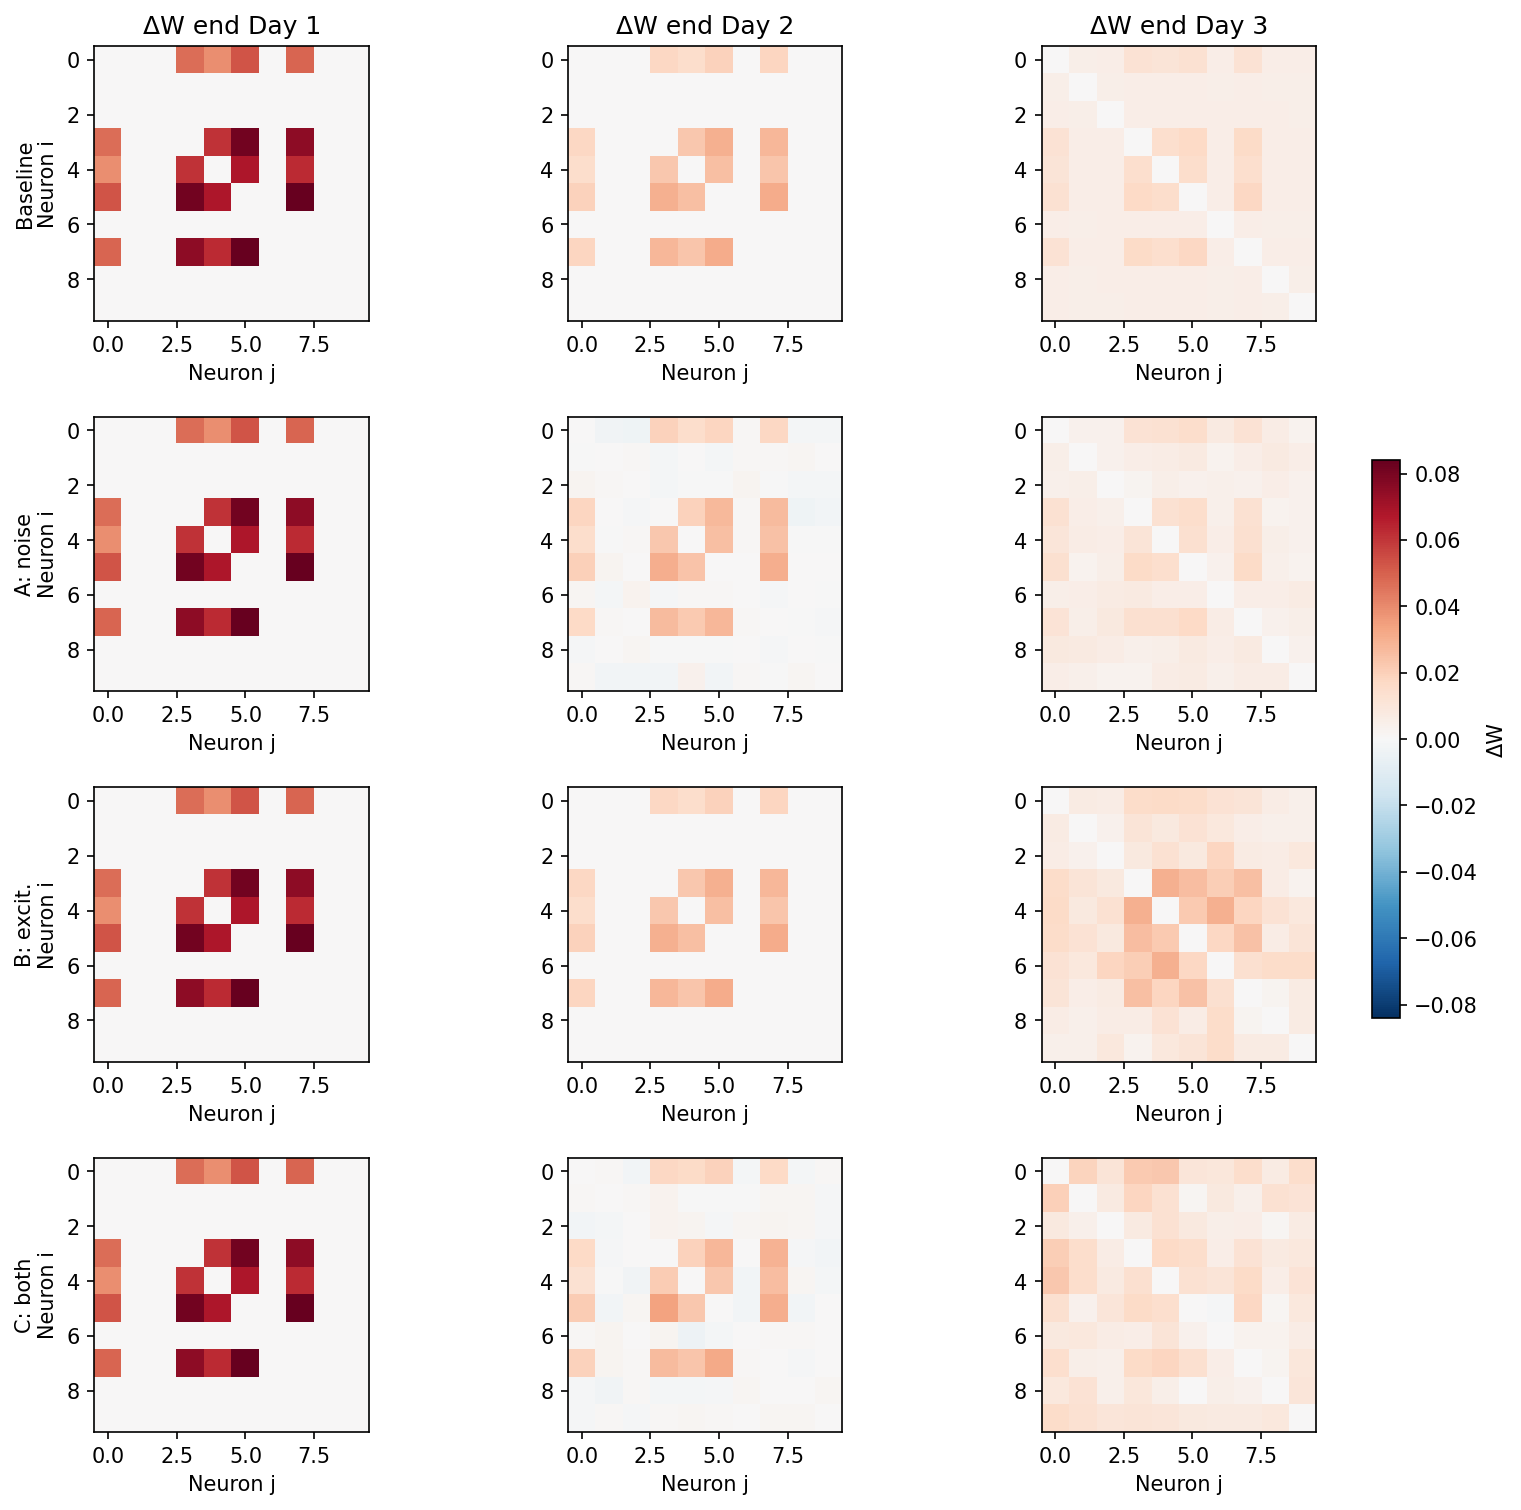
\includegraphics[width=0.97\linewidth]{../figures/fig_W_grid.png}
\caption{\textbf{Weight change $\Delta W = W - W_\mathrm{struct}$ across all conditions and days (one seed).}
Each row is one condition; each column is one day.
Red entries indicate Hebbian potentiation; blue entries indicate sub-baseline weights.
Day~1 (left) is identical across conditions.
Day~2 (middle): passive decay reduces the block uniformly.
Day~3 (right): Baseline and A recover a block consistent with the encoded assembly;
B and C show variable redistribution depending on excitability-driven reactivation order.}
\label{fig:Wgrid}
\end{figure}

\begin{figure}[h]
\centering
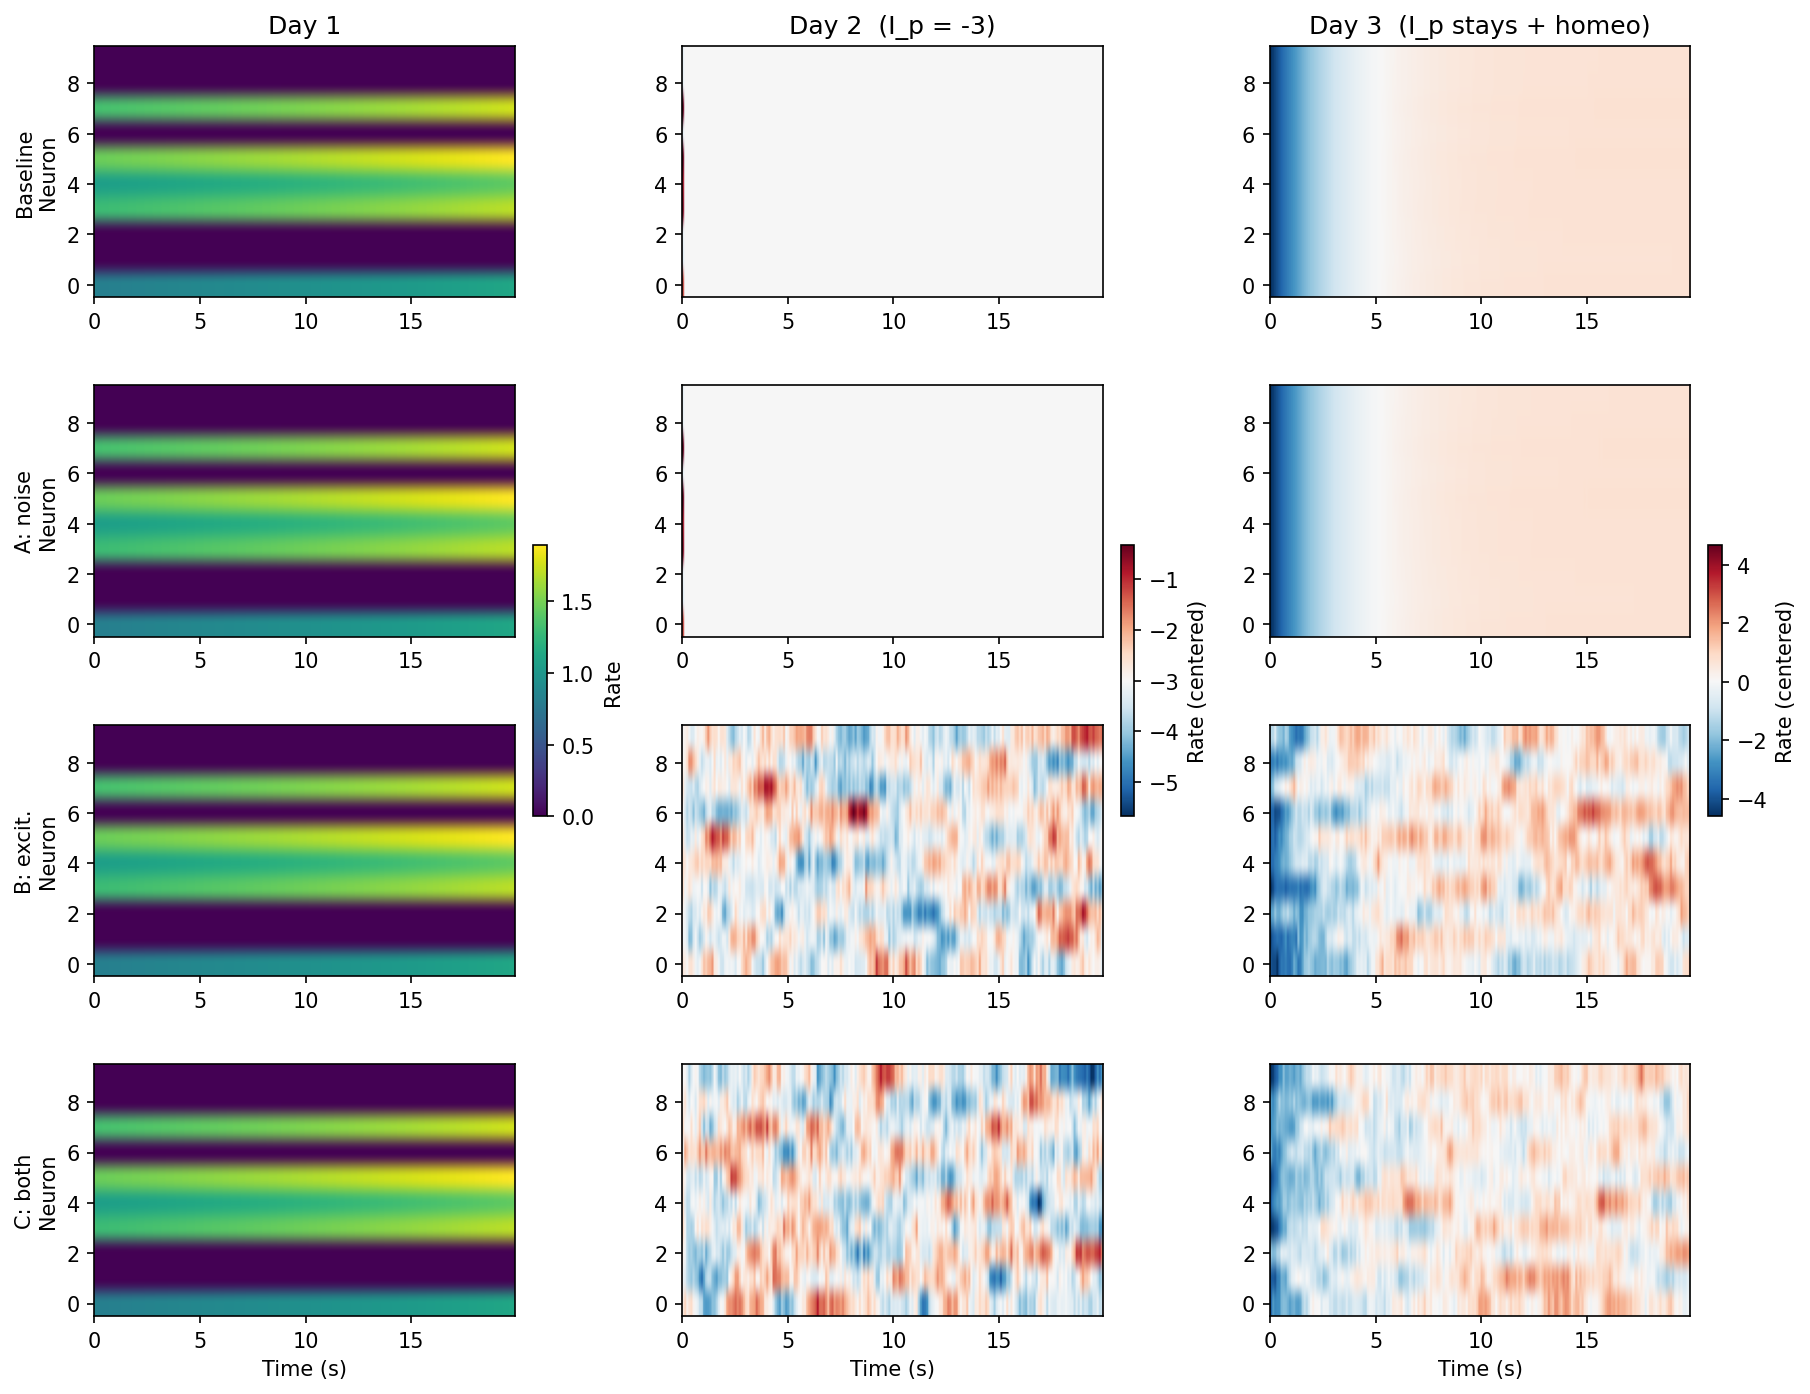
\includegraphics[width=0.97\linewidth]{../figures/fig_activity_heatmaps.png}
\caption{\textbf{Neuron activity heatmaps across all conditions and days (one seed).}
Each row is one condition; each column is one day.
Day~1: five assembly neurons sustain positive rates; five are silent.
Day~2: $I_p=-3$ suppresses all neurons; Baseline and A are uniform (no $\varepsilon_i$),
B and C show OU-driven fluctuations.
Day~3: homeostasis restores activity; pattern structure visible after mean-centering
the colormap per condition.}
\label{fig:activity}
\end{figure}

\begin{figure}[h]
\centering
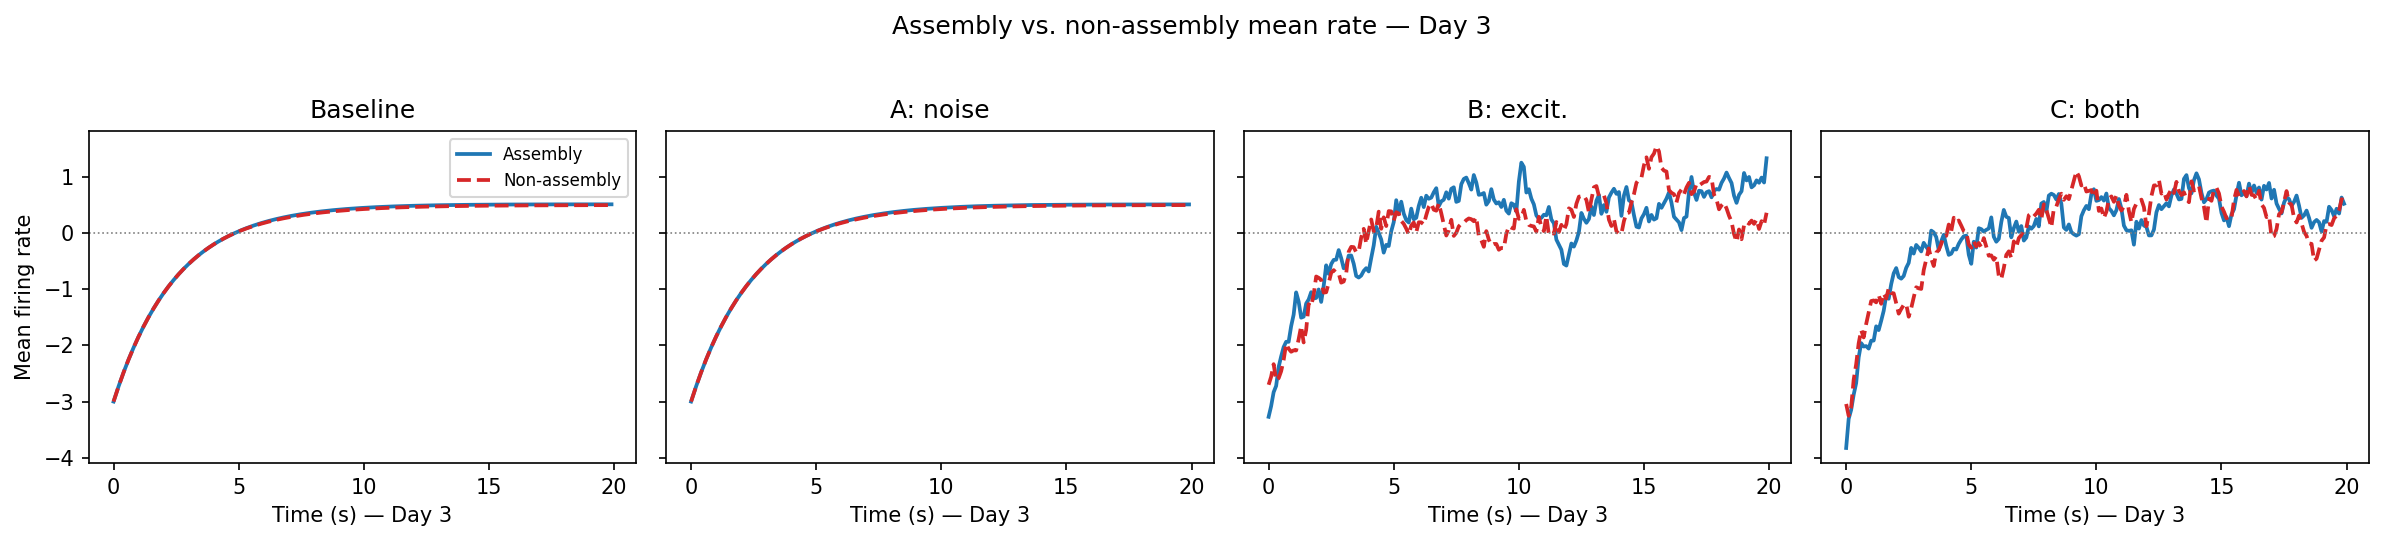
\includegraphics[width=0.97\linewidth]{../figures/fig_assembly_rates.png}
\caption{\textbf{Assembly vs.\ non-assembly mean firing rate during Day~3 (one seed).}
Blue: mean rate of the five assembly neurons. Red dashed: mean rate of the five
non-assembly neurons.  In Baseline and A both groups rise together after the
homeostatic threshold.  In B and C, excitability fluctuations cause differential
reactivation timing; in this seed, B shows the assembly dominating, while C shows
non-assembly neurons competing.}
\label{fig:assembly}
\end{figure}

\begin{figure}[h]
\centering
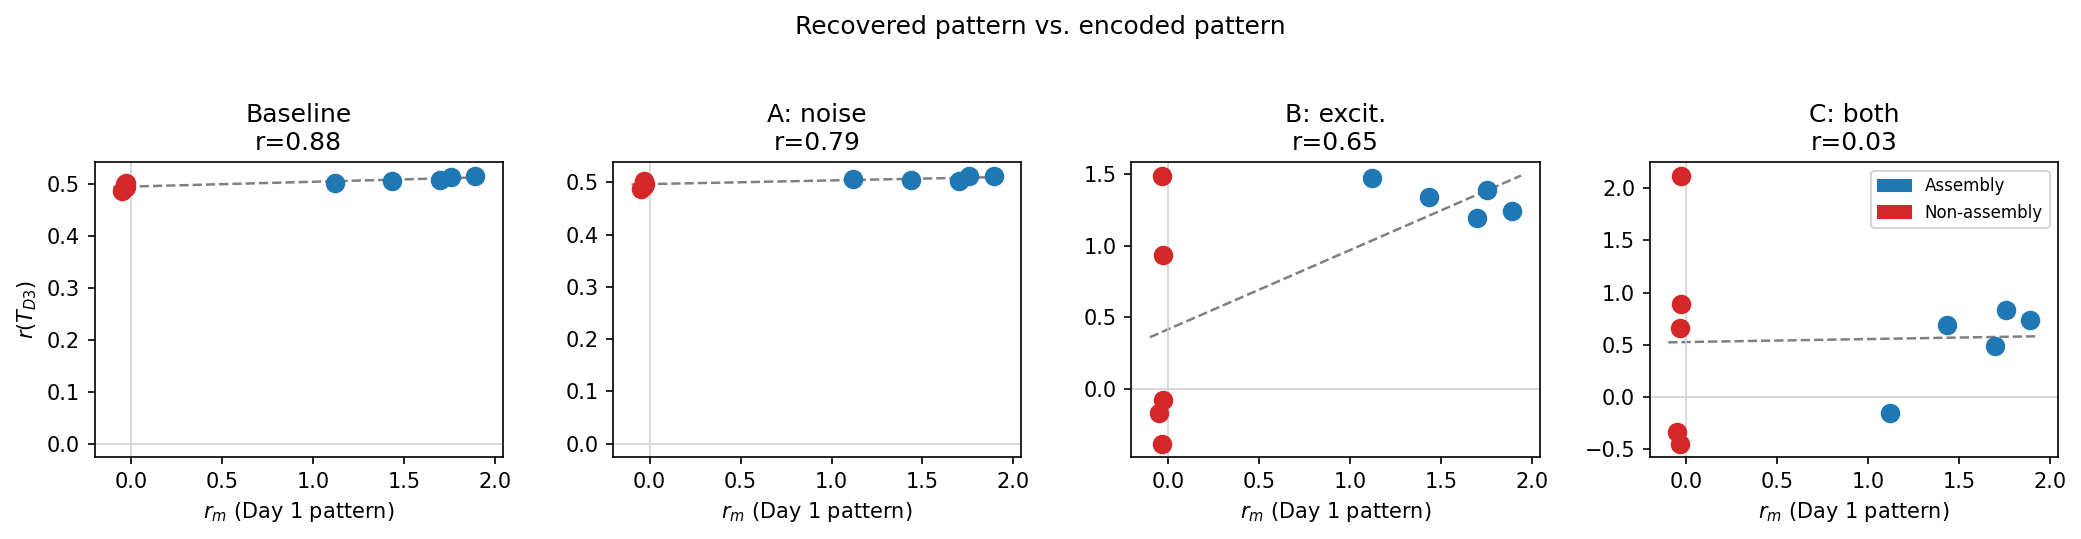
\includegraphics[width=0.97\linewidth]{../figures/fig_pattern_scatter.png}
\caption{\textbf{Recovered vs.\ encoded firing-rate pattern at end of Day~3 (one seed).}
Each point is one neuron; blue = assembly, red = non-assembly.
Pearson $r$ shown in title.
Baseline and A recover near-perfect pattern fidelity ($r\approx0.96$).
B and C show seed-dependent outcomes.}
\label{fig:scatter}
\end{figure}

\begin{figure}[h]
\centering
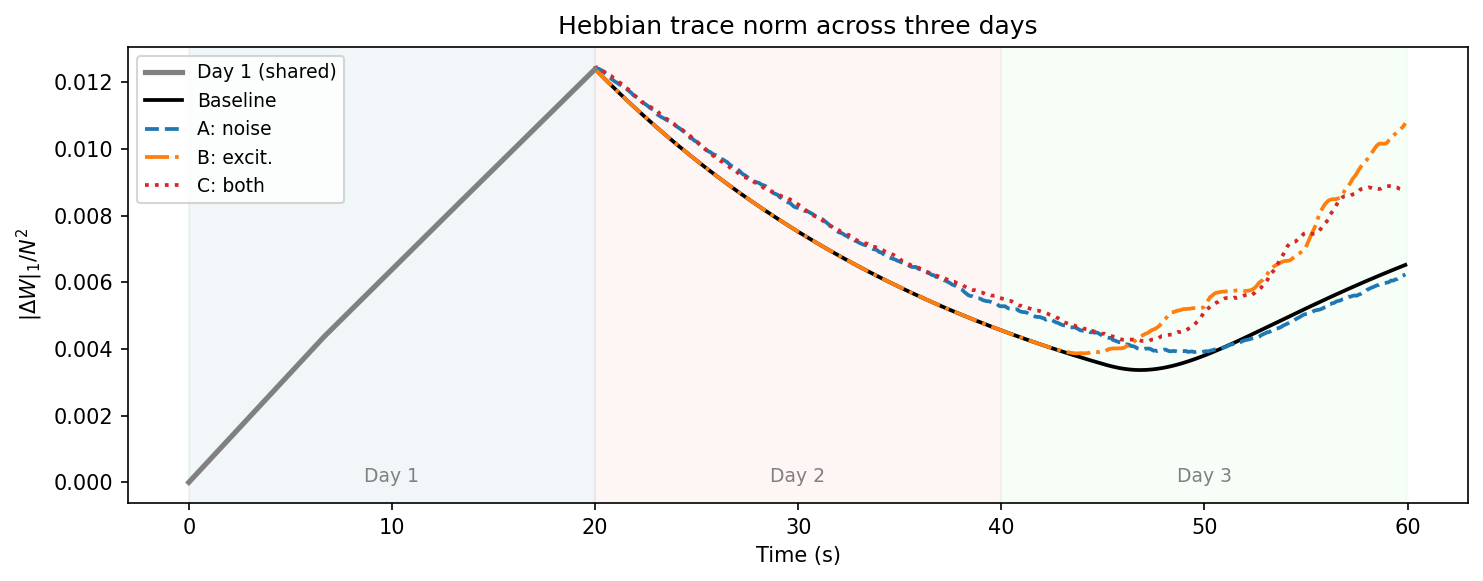
\includegraphics[width=0.85\linewidth]{../figures/fig_trace_norm.png}
\caption{\textbf{Hebbian trace norm $|\Delta W|_1/N^2$ across the three-day protocol (one seed).}
Gray: Day~1 shared.  Colored lines: individual conditions from Day~2 onward.
The trace decays during Day~2 and diverges on Day~3 depending on which neurons
reactivate and get Hebbian reinforcement.}
\label{fig:trace}
\end{figure}

% ================================================================
\section{Discussion}

Our simulations reveal a clear functional dissociation between the two noise
sources.  Synaptic noise on $\dot{W}$ ($\sigma_\eta = 0.01$) has negligible
effect on memory recovery: it neither shifts the mean $m_\mathrm{mem}$ nor
introduces variability.  This is consistent with the magnitude being well below
the threshold that would destabilise the assembly attractor \citep{Qin2023}.

Slow intrinsic excitability fluctuations, by contrast, introduce a
\emph{stochastic bifurcation}: the network has two possible fates
(correct assembly vs.\ spurious pattern), and which one is realized depends
entirely on the random OU trajectory at the moment of homeostatic reactivation.
This is the key result.  The mechanism is simple: the homeostatic drive $h(t)$
is scalar and raises all neurons uniformly, so the \emph{order} of reactivation
is determined solely by $\varepsilon_i$ heterogeneity.  Neurons with large
positive $\varepsilon_i$ cross zero first and receive the first Hebbian
potentiation.  If these happen to be assembly neurons, the correct pattern is
reinforced; if they are non-assembly neurons, a spurious pattern can become
self-sustaining before the true assembly activates.

This mechanism is directly linked to representational drift: across days, the
random walk of $\varepsilon_i$ progressively changes which neurons reactivate
first, gradually shifting the represented pattern \citep{Delamare2023}.
Our model shows that a single episode of suppression and homeostatic rescue is
sufficient to produce this shift in a measurable way, even without ongoing
experience-dependent plasticity.

Slow fluctuations in intrinsic conductances \citep{Delamare2023} are one
biological source of excitability heterogeneity; our results predict that
in the presence of such fluctuations, homeostatic rescue can be faithful or
catastrophically wrong with roughly equal probability, depending only on
the phase of the excitability fluctuations at the time of reactivation.
This is consistent with experimental observations that representational drift
is highly variable across sessions even under controlled conditions \citep{Bauer2024}.

The finding that homeostasis restores mean firing rates in all conditions
($m_\mathrm{mean}\approx0.5$, $h\approx3.5$) but does so to variable patterns
in B and C demonstrates that homeostatic rate recovery is \emph{necessary but
not sufficient} for memory fidelity---a point also noted in theoretical work
on homeostatic stabilization \citep{DarshanRivkind2022}.

\paragraph{Code availability.}
All simulation code, notebooks, and figures are available at
\url{https://github.com/eegoro/representational-drift}.

\paragraph{Limitations and outlook.}
The small network ($N=10$) limits capacity to one stored pattern.  With larger
$N$, one could test whether excitability fluctuations preferentially bias recall
toward more recently encoded memories.  A per-neuron homeostatic controller
(rather than scalar $h$) could compensate for excitability heterogeneity and
reduce the variance of outcomes.  Finally, the Euler stability window limits
encoding duration; a normalised Hebbian rule \citep{Qin2023} would allow longer
simulations and multiple stored patterns.

\clearpage
\bibliographystyle{abbrvnat}
\bibliography{refs}

\end{document}
